\documentclass{article}
\usepackage{amsmath}
\usepackage{siunitx}
\usepackage{xcolor}
\usepackage{hyperref}
\usepackage{graphicx}
\usepackage{listings}
\lstset{language=Python,%
	basicstyle=\footnotesize\ttfamily,stringstyle=\color{red!40!black},%
	commentstyle=\color{violet!95!black}\textsf,%
	keywordstyle=\color{green!30!black}, morekeywords={as},%
	tabsize=3,breaklines=true,postbreak=\mbox{\textcolor{red}{$\hookrightarrow$}\space}, showstringspaces=false,%
	backgroundcolor = \color{black!3!white}}
\usepackage[a4paper, left=2cm, right=2cm, top=2cm, bottom=2cm]{geometry}

\author{Marco Codato}
\title{Notes}

\begin{document}
\maketitle

\section{Introduction}

Moved to the GitHub repository  \href{https://github.com/codatomrc/tesi}{\texttt{codatomrc/tesi}}.

\section{Background spectrum extraction}

\subsection{Automatic detection}
The script I am writing works as follows.
\begin{itemize}
	\item Automatically explores a directory and find all the raw files, marked as \texttt{filename.fc.fits}. All the files are then processed one by one.
	
	\item Far each frame relevant information is extracted from the header (hdr). In particular the script requires
	\begin{itemize}
		\item information about the wavelength of each pixel (initial wavelength, increment of each pixel and width of the detector and horizontal binning factor),
		\item slit width and length (thus the detector height an vertical binning factor, aside the CCD scale),
		\item year of observation
	\end{itemize}
	\item For each frame a preliminary integration over all the wavelenghts is performed by summing the data in the file along the dispersion direction. This is an efficient way of detecting astronomical sources, that are spatially limited, against the background, supposed uniform along the slit.
	
	\item I estimate the noise level and amplitude for the slit luminosity profile by comparing the original profile with a detrended version.
	I used a biweighted detrending algorithm with a windowing of 10 times the slit width, using the function \href{https://github.com/hippke/wotan}{\texttt{wotam.flatten}}
	The choice of such a wide widow (about 40\,px for a typical \SI{100}{\micro\metre} slit size) allows us to have a good compromise to estimate both noise level and amplitude:
	\begin{itemize}
		\item bkg level is the average value of the detrended profile. This is a good estimation of the real value since I used a large window and the light of the bright peaks is smeared on a wide area, making its contribution less relevant.
		\item noise amplitude is the standard deviation of the original profile wrt the detrended one.
	\end{itemize}
	Note choosing a wider window improves the estimation of the bkg level (even if it cannot actually ever converge to the real value) but increases the estimated noise amplitude.
	
	\item Cosmic rays and excessive noise are removed. In particular in the bluer part of the spectrum, due to the low sensitivity of the detector, after the flux calibration the noise is extremely high, seriously affecting the quality of the measurements. For example see the image below
	\begin{figure}[h!]
		\centering
		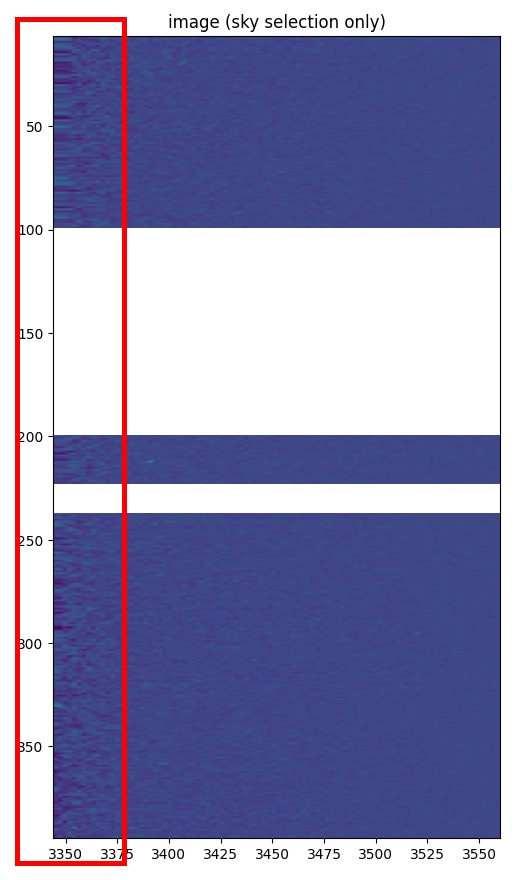
\includegraphics[width=.35\textwidth, angle=90]{10_det}
	\end{figure}
	I removed these features by scanning each column of the frame looking for bright sharp peaks. Some good settings to remove both cosmic rays and noise is to find peaks very thin, with a width less than 3\,px and an height of more than 5 times the average level of the bkg (i.e.\ the value estimated from the luminosity profile, divided by the number of pixels along the horizontal direction) \textcolor{red}{bisognerebbe stimare la dimensione apparente dei raggi cosmici e confrontarla con la scala sul CCD per essere sicuri che funzioni con tutte le immagini}.
	
	The peaks were identified with the function \href{https://docs.scipy.org/doc/scipy/reference/generated/scipy.signal.find_peaks.html}{\texttt{scipy.signal.find\_peaks}} while their FWHM was estimated with \href{https://docs.scipy.org/doc/scipy/reference/generated/scipy.signal.peak_widths.html#scipy.signal.peak_widths}{\texttt{scipy.signal.peak\_widths}}. To be sure all the cosmic ray trace or the noise fluctuation was contained in the detected width I added a further 1\,px on both directions along the columns.
	
	\item On the cleaned frame I take again luminosity profile along the slit (i.e.\ integration on the wavelengths) to search for the astronomical sources. I used \texttt{scipy.signal.find\_peaks} to find the position of the sources. I selected only those features with a width larger than 3\,px (to be sure not to include unremoved cosmic rays) and with a \href{https://en.wikipedia.org/wiki/Topographic_prominence}{prominence} equal to the estimated noise amplitude.
	
	\item I computed the width of the sources with \texttt{scipy.signal.peak\_widths}. In particular I considered the FWHM which proved to be more solid than the total width. Since many kinds of astronomical sources have a central core and bright wings, I decided to remove a that span $3\times\text{FWHM}$ wrt the center of the peak to take into account such wings.	
	
	\item At the end the script produces:
	\begin{itemize}
		\item A plot of the luminosity profile along the slit (the one from the original frame, and after the cosmic ray removal) plus the masked source regions.
		\item The bkg spectrum from the selected rows only, integrated along the spatial direction (plus the same for the full cleaned frame as a comparison).
		\item A new file where cosmic rays, the UV noise and the astronomical sources are removed. The information in the hdr are preserved and the data when the file was produced is added.
	\end{itemize}
\end{itemize}


\paragraph{A quantitative approach.} I tried to sketch a qualitative model where I assumed gaussian profiles of the sources. The source ended when its flux was comparable to the amplitude of the bkg noise. The final distance $\Delta$ from the center of the source was
\[\Delta = \frac{1}{2\sqrt{2\ln 2}}\text{FWHM}\sqrt{\ln(S_\text{max}^2/B)}   \]
where $S_\text{max}$ was the maximum counts of the source, while $B$ the average level of bkg around the object. Since many extended objects cannot be reproduced by gaussian profiles this estimation may be misleading in many cases. Since the empirical procedure discussed above seems quite solid with current data, implementing a rigorous analytical approach that accounts for different luminosity profiles of the sources, is definitively unecessary.

\subsection{Preliminary results}
Here I report some relevant results I obtained.

\paragraph{All the data.} Wavelength integrated profiles and bkg-removed spectra obtained with the current configuration are available in the directories \texttt{plots/integr} and \texttt{plots/sky\_spec} respectively. The masked spectra are saved in the same directories of the original files with syntax \texttt{filename.fc.bkg.fits}.

\paragraph{IMA06889 (2009).} A extremely high signal is present in the bluer part of the spectrum. Anyway the wavelengths are extremely low (below \SI{3000}{\angstrom}) and these are not very relevant.
\begin{figure}[h!]
	\begin{minipage}{.49\textwidth}
		\centering
		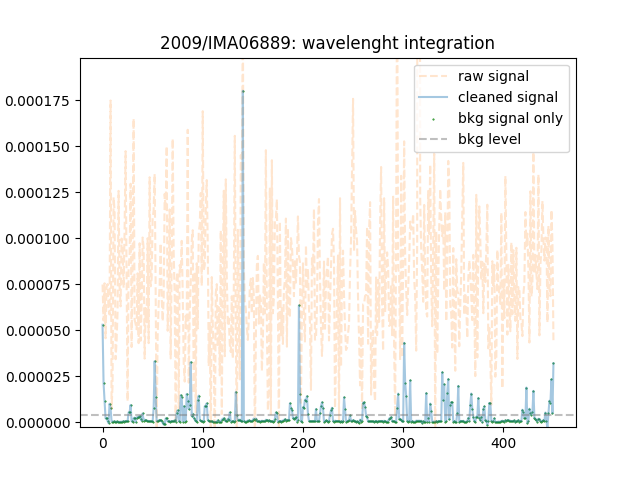
\includegraphics[width=\textwidth]{2009_IMA06889}
	\end{minipage}
\hfill
	\begin{minipage}{.49\textwidth}
	\centering
	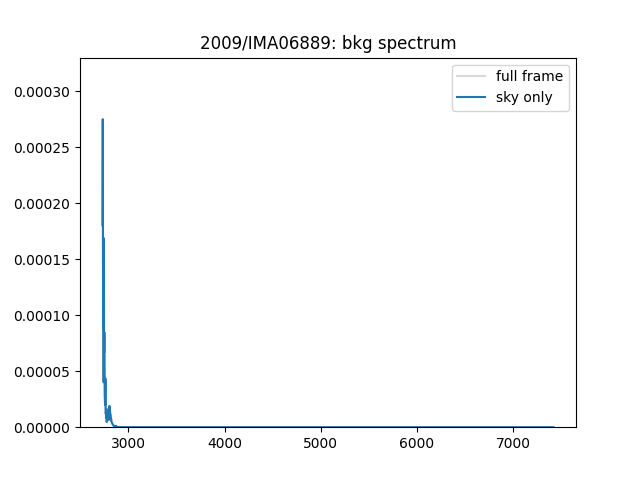
\includegraphics[width=\textwidth]{IMA06889}
\end{minipage}
\end{figure}
We realize that the original profile along the slit was severely noisy and after the cleaning there is still some residual noise that makes the profile very irregular.

\paragraph{IMA91077 (2020) and others.} In this case we notice that the profile of the bkg is not uniform at all but seems to present a systematic trend. I need to investigate if it is intrinsic (e.g.\ due to a diffuse component) or the result of some calibration or instrumental issue.
\begin{figure}[h!]
		\centering
		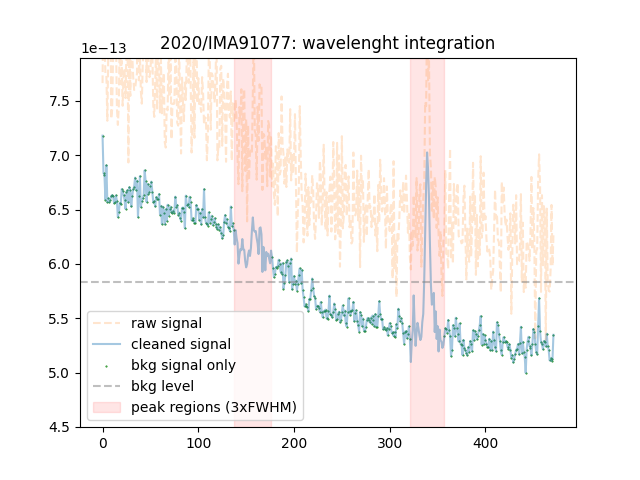
\includegraphics[width=.49\textwidth]{2020_IMA91077}
\end{figure}
Similar features are presents in other frames like IMA61434 (2017), IMA84983, IMA85634, IMA91077 (2020), IMA95725 and IMA97134 (2021).

\subsection{Comments on the first results}

\paragraph{Wavelength limitations.} It would be convenient to set a wavelength threshold for the analyzed data. Wavelengths outside the spectrograph+telescope working range may led to biased measurements. Due to the strong noise in the bluer part of the spectrum, many of such portion of the images is automatically masked, but probably some of the inconsistent results are due to such noise.

\paragraph{Frame limitations(?)} I wonder whether the whole CCD area is suitable for collecting data or it would be better/necessary to neglect some specific regions, both in the spatial and dispersion directions.

\textcolor{red}{What about the lines ``\texttt{CCDSEC}'' and ``\texttt{BIASSEC}'' in the header of the frames?}

\newpage
\section{Appendix: Python source code}
The code I am using.
\lstinputlisting[language=Python]{../bkg_extractor.py}

\end{document}

